\chapter{Methoden}

% Aus Aufbau_Bericht.pdf
% Hier halten Sie fest und begründen, welches Vorgehensmodell Sie für Ihr Projekt wählen. Sie
% verweisen allenfalls auf die daraus entstandenen, konkreten Terminpläne mit Meilensteinen, welche
% z.B. unter Realisierung (Kapitel 5) oder im Anhang versorgt sind.

% Bei Engineering-Projekten halten Sie weitere einzusetzende fachliche Methoden oder Techniken fest.
% Bei einem Softwareprojekt können dies z.B. der geplante Einsatz einer Anforderungsanalyse, der
% Einsatz von Review-Techniken (Architektur-Reviews) oder bekannter Programmiertechniken sein.


% TODO evtl einleitung schreiben


\section{Vorgehensmodell}\label{vorgehen}
In der Aufgabenstellung (Anhang \ref{anhang:aufgabenstellung}) wurde verlangt, das der Scrum Prozess, so wie er bei der Landis+Gyr gelebt wird, als Vorgehensmodell verwendet wird.
Diverse Eigenschaften und Abläufe dieses Prozesses konnten direkt für diese Arbeit übernommen und angewandt werden.
Da an dieser Arbeit nur ein Entwickler arbeitet und auch die Anzahl Stakeholders kleiner ist, wurden mehrere Dinge angepasst.
Die folgenden Abschnitte geben einen Überblick über den Prozess, wo sich dieser von jenem der Landis+Gyr unterscheidet und wieso diese Anpassungen vorgenommen wurden.

\subsection{Sprints}
Das Projekt besteht aus mehreren aufeinanderfolgenden Sprints.
Jeder Sprint dauert zwei Wochen.
Während eines Sprints wird an jenen User Stories gearbeitete, welche für diesen Sprint eingeplant sind.
Die Entwickler geben zu Beginn des Sprints das Commitment ab, dass sie die geplanten Stories im Sprint abschliessen werden.
Um weder zu viele noch zu wenige Stories in einem Sprint zu planen, wird bei der Landis+Gyr jeder Story eine Wert gegeben.
Dieser Wert, welcher Story Points genannt wird, wird von den Entwicklern geschätzt und beziffert den erwarteten Aufwand.
Auf Story Points wurde bei dieser Arbeit verzichtet, da sie für den Einzelentwickler keinen Mehrwert bieten.

Während die Dauer aller Sprints genau gleich ist, variiert die Zeit, welche der Entwickler für Entwicklungsarbeiten aufwenden kann, von Sprint zu Sprint stark.

\subsubsection{User Story}\label{userstory}
Der Scrum Prozess der Landis+Gyr kennt viele unterschiedliche Work Items wie z.B. Epics, Requirements oder Features.
In Abbildung \ref{fig:workitems} sind sie alle dargestellt.
\begin{figure}[H]
   \centering
   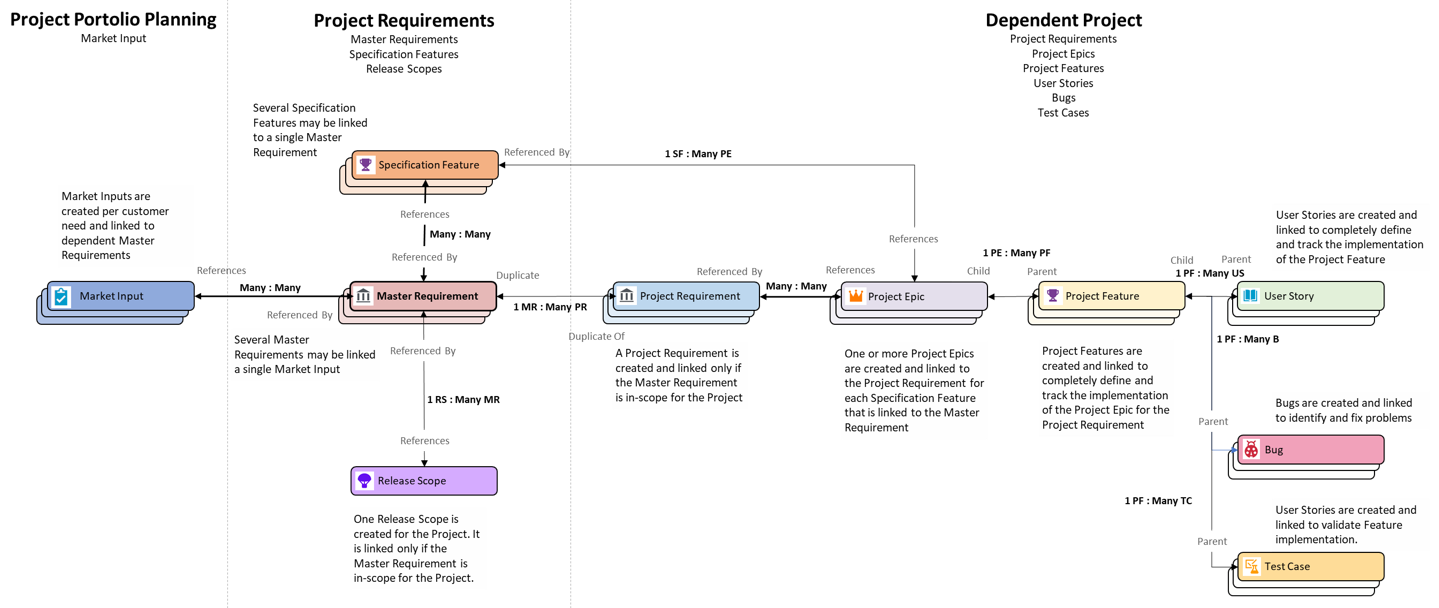
\includegraphics[width=1.0\textwidth]{gfx/WorkItemRelationsship.png}
   \caption{
      Übersicht über die verschiedenen Work Items im Scrum Prozess der Landis+Gyr
      }
      \label{fig:workitems}
\end{figure}
Um möglichst wenig Zeit mit administrativen Aufgaben zu verbrauchen, werden für diese Arbeit nur User Stories eingesetzt.
Eine User Story beschreibt jeweils ein Arbeitspaket, welches während eines Sprints vollständig bearbeitet werden kann.
Sie enthält eine Sammlung von Akzeptanzkriterien, welche durch die Bearbeitung der Story erfüllt werden müssen.
Damit eine Story als fertig gilt, muss die Definition of Done erreicht werden. Diese wird im folgenden Abschnitt erläutert.

%todo task?

\subsubsection{Definition of Done}
Für diese Arbeit besteht die Definition of Done aus folgenden Punkten:
\begin{itemize}
   \item Alle Akzeptanzkriterien sind erfüllt.
   \item Unittests wurden implementiert oder angepasst, decken mindestens 80\% des Codes ab und laufen erfolgreich durch.
   \item Der Code entspricht dem Coding Style, siehe \ref{codingStandard}.
\end{itemize}

Bei der Landis+Gyr gehört zur Definition of Done zusätzlich noch, dass der Code von mindestens zwei weiteren Entwicklern gegengelesen wurde.
Dies ist bei diesem Projekt leider nicht möglich.


\subsection{Meetings}
Zum Scrum Prozess der Landis+Gyr gehören diverse Meetings, welche regelmässig stattfinden.
So wird ein Sprint jeweils im Voraus während des \textit{Sprint Planning} geplant.
Während des Sprints findet im \textit{Daily Meeting} ein täglicher Austausch zwischen allen Entwicklern statt.
Im \textit{Sprint Review} werden nach einem Sprint die erarbeiteten Stories präsentiert.
Die \textit{Retrospektive}, welche ebenfalls nach jedem Sprint stattfindet, regt die Entwickler dazu an, die eigenen Arbeitsprozesse zu reflektieren und diese womöglich zu verbessern.

Alle diese Meetings werden für diese Arbeit weggelassen.
Die Planung des neuen Sprints wird jeweils ad hoc erledigt und Änderungen am Arbeitsprozess sofort umgesetzt.
Während des Projekts finden mehrere Meetings mit der Betreuungsperson dieser Arbeit statt.
Dort werden jeweils die gemachten Fortschritte und erledigten Arbeiten präsentiert.
Somit lassen sich diese teilweise mit dem \textit{Sprint Review} vergleichen.
Sie sind zeitlich jedoch nicht an die Sprints gebunden.

\subsection{Rollen}
Bei der Landis+Gyr besteht jedes Entwicklungsteam aus mehreren Entwicklern und ein bis zwei Testern.
Eine dieser Personen übernimmt zusätzlich die Rolle des Scrum Master.
Dieser ist für die Organisation und Durchführung der zuvor genannten Meetings verantwortlich.
Eine weitere Rolle ist der Produkt Owner.
Dieser erstellt und verwaltet die User Stories im Backlog.

Für diese Arbeit werden die Rollen des Entwickler, Tester, Scrum Master und Product Owner in einer einzigen Person vereint.


\section{Azure DevOps}\label{methoden:ADO}
Bei der Landis+Gyr wird \ac{ADO} für die Verwaltung des Scrum Backlogs eingesetzt.
In der Software können die Work Items, welche im Abschnitt \ref{userstory} aufgezeigt werden, verwaltet werden.
Für dieses Projekt soll \ac{ADO} verwendet werden, um die einzelnen Sprints zu planen.
\begin{figure}[H]
   \centering
   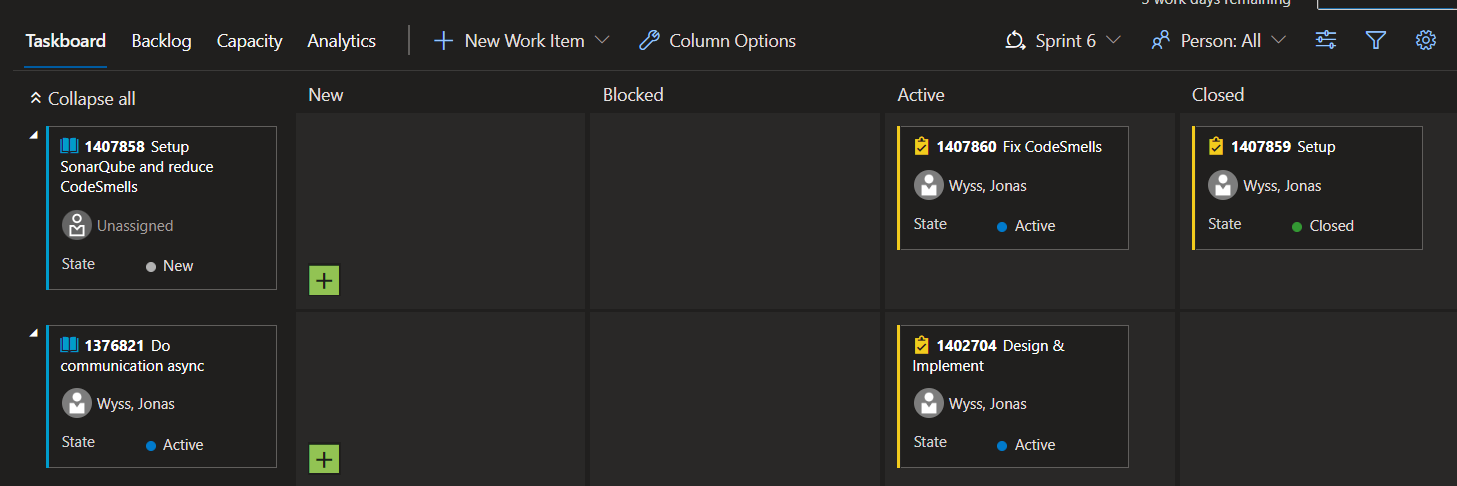
\includegraphics[width=1.0\textwidth]{gfx/ado.png}
   \caption{
         Ausschnitt aus dem Backlog des sechsten Sprints in \ac{ADO}
      }
      \label{fig:adosprint6}
\end{figure}
Wärend der Sprints soll das aktuelle Backlog jeweils einen Überblick über den aktuellen Stand der Arbeiten geben.
In Abbildung \ref{fig:adosprint6} ist gezeigt, wie dies ausschauen kann.

Zusätzlich sollen zwei weitere Funktionen von \ac{ADO} verwendet werden:
\begin{itemize}
   \item Der Quellcode soll in einem Repository abgelegt werden, welches von \ac{ADO} verwaltet wird.
   \item Die Pipelines von \ac{ADO} sollen für \ac{CICD} verwendet werden.
\end{itemize}

\section{Coding Style}\label{codingStandard}
In Abschnitt \ref{quality_richtline} ist beschrieben, wie das Befolgen einer Software-Richtlinie einen positiv Effekt auf die Codequalität haben kann.
Der C\# Code, der für diese Arbeit geschrieben wird, soll den Coding Style der dotnet runtime \footnote{https://github.com/dotnet/runtime/blob/main/docs/coding-guidelines/coding-style.md} befolgen.
Die Entwicklungsumgebung Visual Studio ist standardmässig so konfiguriert, dass sie diesem Style folgt.
Sie unterstützt die Entwickler mit automatischen Formatierungen und weist auf Verletzungen des Standards hin.

\section{Test Driven Development} \label{tdd}
\ac{TDD} ist ein Vorgehen bei dem Produktiv- und Testcode parallel geschrieben werden.
Dabei wird jeweils zuerst ein Testfall geschrieben, welcher fehlschlagen soll.
Danach wird genau so viel Code geschrieben, dass der Testfall abgedeckt ist.
Nun kann der geschriebene Code wenn nötig überarbeitet werden.
Bestehende Testfälle dürfen nicht gebrochen werden.
Dieses Vorgehen wird solange wiederholt, bis alle benötigten Funktionen getestet und implementiert sind.
Ein Vorteil von \ac{TDD} ist, dass die Entwicklungsarbeit vorhersagbar wird.
Ist eine Funktion implementiert, kann mit Sicherheit gesagt werden, dass diese auch richtig funktioniert \parencite{beck2003test}.
Mit diesem Vorgehen wird auch sichergestellt, dass die Testbarkeit (mehr dazu in Abschnitt \ref{testability}) einer Komponente gut ist.

In dieser Arbeit soll wenn immer möglich nach \ac{TDD} vorgegangen werden.


\section{Diagramme}
Diagramme, welche während des Designprozesses erstellt werden, sollen mit PlantUML\footnote{https://plantuml.com/} erstellt und dem UML Standard folgen.
Dies gilt auch für jene Diagramme, die in dieser Arbeit aufgeführt werden.